\documentclass[twocolumn]{svjour3}

\usepackage[T1]{fontenc}
\usepackage[utf8]{inputenc}
\usepackage{mathptmx}
\usepackage{amsmath}
\usepackage{graphicx}
\usepackage{booktabs}
\usepackage{array}
\usepackage{url}

\graphicspath{{figures/}}
\journalname{Journal of Artificial Life and Robotics}

\begin{document}

\title{Blood Pressure Estimation from 30 fps Visible-Light rPPG Using an Asymmetric Sine Wave Model}
\titlerunning{Asymmetric Sine Model for 30 fps rPPG BP Estimation}

\author{Yusuke Nakazawa \and Kento Nagumo \and Akio Nozawa}
\authorrunning{Y. Nakazawa et al.}

\institute{
Y. Nakazawa \at
Department of Electrical and Electronic Engineering, Graduate School of Science and Engineering, Aoyama Gakuin University, Sagamihara, Japan \\
Corresponding author \\
Tel.: +81-80-5326-3916 \\
Fax: Not available \\
\email{nynynakazawa@gmail.com}
\and
K. Nagumo \at
Department of Electrical and Electronic Engineering, Graduate School of Science and Engineering, Aoyama Gakuin University, Sagamihara, Japan
\and
A. Nozawa \at
Department of Electrical and Electronic Engineering, Graduate School of Science and Engineering, Aoyama Gakuin University, Sagamihara, Japan
}

\date{}

\maketitle

\begin{abstract}
Continuous blood pressure monitoring with consumer smartphones is attractive for home healthcare, but 30 fps visible-light cameras provide coarse pulse-wave sampling and unstable beat morphology. Under this constraint, point-based features such as peak timing are easily disturbed by frame quantization and illumination noise. This study evaluates an asymmetric sine wave model as a low-parameter time-domain representation for remote photoplethysmography (rPPG) and compares three estimators: a morphology-based baseline (RTBP), a fitted-parameter model [sinBP(M)], and a residual-aware model [sinBP(D)] that augments RTBP features with the asymmetric-sine residual $E$. Using the prepared repository dataset of 469 beat-level samples with synchronized systolic and diastolic blood pressure references across 11 recording groups, model fitting reduced waveform MAPE from 29.71\% to 18.22\%. In the cleaned five-fold time-series re-evaluation, sinBP(D) achieved the lowest mean absolute-error values, with MAE/RMSE of 18.96/24.16 mmHg for systolic pressure and 14.80/19.28 mmHg for diastolic pressure. However, recording-group-aware validation showed that absolute cross-group estimation remained weak, especially for systolic pressure. By contrast, in a grouped trend-oriented reanalysis with group-centered targets and 20~s non-overlapping windows, sinBP(D) yielded the best systolic trend result, with MAE/RMSE of 3.22/3.90~mmHg. These results support the asymmetric sine representation more strongly as a trend-oriented descriptor under 30 fps visible-light conditions than as a standalone absolute blood-pressure estimator.
\keywords{Blood pressure estimation \and remote photoplethysmography \and smartphone camera \and waveform modeling \and residual analysis}
\end{abstract}

\section{Introduction}
Continuous and non-invasive blood pressure (BP) monitoring remains an important goal for preventive medicine and daily health management \cite{Whelton2018,Sun2016}. Smartphone-based photoplethysmography (PPG) is attractive because it is inexpensive, familiar to users, and does not require dedicated sensing hardware \cite{Sun2016,Verkruysse2008}. However, most consumer-facing visible-light camera pipelines still operate at 30 fps, where one frame corresponds to about 33 ms. In this regime, peak and valley positions are sampled coarsely, morphological features fluctuate, and high-order harmonic analysis becomes unreliable \cite{Millasseau2006,Alian2014,McDuff2014}.

The methodological question addressed here is whether a low-parameter whole-wave model is more stable than point-based morphology under this sampling constraint. The asymmetric sine model was selected because it can represent the rapid systolic rise and slower diastolic decay of a fingertip pulse with only a few parameters. This design avoids relying on higher-order decomposition terms that are difficult to estimate robustly from 30 fps data.

This paper compares three estimators derived from the same preprocessing pipeline: a point-feature baseline (RTBP), a fitted-parameter model [sinBP(M)], and a residual-aware hybrid model [sinBP(D)] that adds the fit residual $E$ to the RTBP feature set. The goal is not to claim clinical readiness, but to examine whether whole-wave fitting yields a more stable representation for BP estimation in low-frame-rate visible-light rPPG. In particular, we ask two practical questions: whether the fitted-wave representation improves the aggregate absolute-error metrics reported in the repository, and whether it more reliably tracks within-recording BP variation than the point-feature baseline.

\section{Related Work}
Many BP-estimation studies from PPG use point-derived morphology, timing surrogates, or hybrid feature sets that combine amplitude ratios, rise-time ratios, and other beat landmarks \cite{Sun2016,Alian2014,Finnegan2023,Fleischhauer2022}. These approaches are useful when fiducial points are sampled reliably, but their stability deteriorates when peaks and valleys move by one or two frames. This issue is especially relevant for visible-light smartphone acquisition at 30 fps, where the sampling interval is already comparable to short systolic sub-phases. Pulse decomposition and higher-order waveform analysis can recover richer shape information, yet they also become fragile when the beat is sparsely sampled or corrupted by illumination noise \cite{Millasseau2006,Allen2007,Hall2020}.

Recent rPPG-based BP work has increasingly used higher-dimensional learning pipelines or whole-wave representations rather than only hand-picked landmarks. Examples include remote-PPG ensemble regression \cite{vanPutten2023}, robust waveform-level modeling of pressure reconstruction from contact PPG \cite{Pan2024}, and trend-oriented systolic BP estimation that explicitly separates within-recording fluctuation from cross-subject level differences \cite{Huang2025}. These studies motivate two points for the present work. First, representation choice matters when waveform quality is limited. Second, trend estimation and absolute cross-group estimation should be treated as distinct tasks. The present study is therefore positioned narrowly: it does not claim a broad benchmark win, but instead tests whether a compact asymmetric-sine representation is more stable than RTBP-style point morphology under low-frame-rate visible-light sampling.

\section{Methods}
\subsection{Overall Approach}
Figure~\ref{fig:overview} summarizes the processing flow. A fingertip video is recorded with a smartphone front camera, converted to a pulse-like waveform, segmented beat by beat, and then passed to three estimators that share the same preprocessing. RTBP uses morphology-derived features from the original beat sequence. sinBP(M) uses low-parameter descriptors from the asymmetric sine fit. sinBP(D) reuses the RTBP feature set and adds the residual error between the measured beat and the fitted waveform.

\begin{figure}[t]
\centering
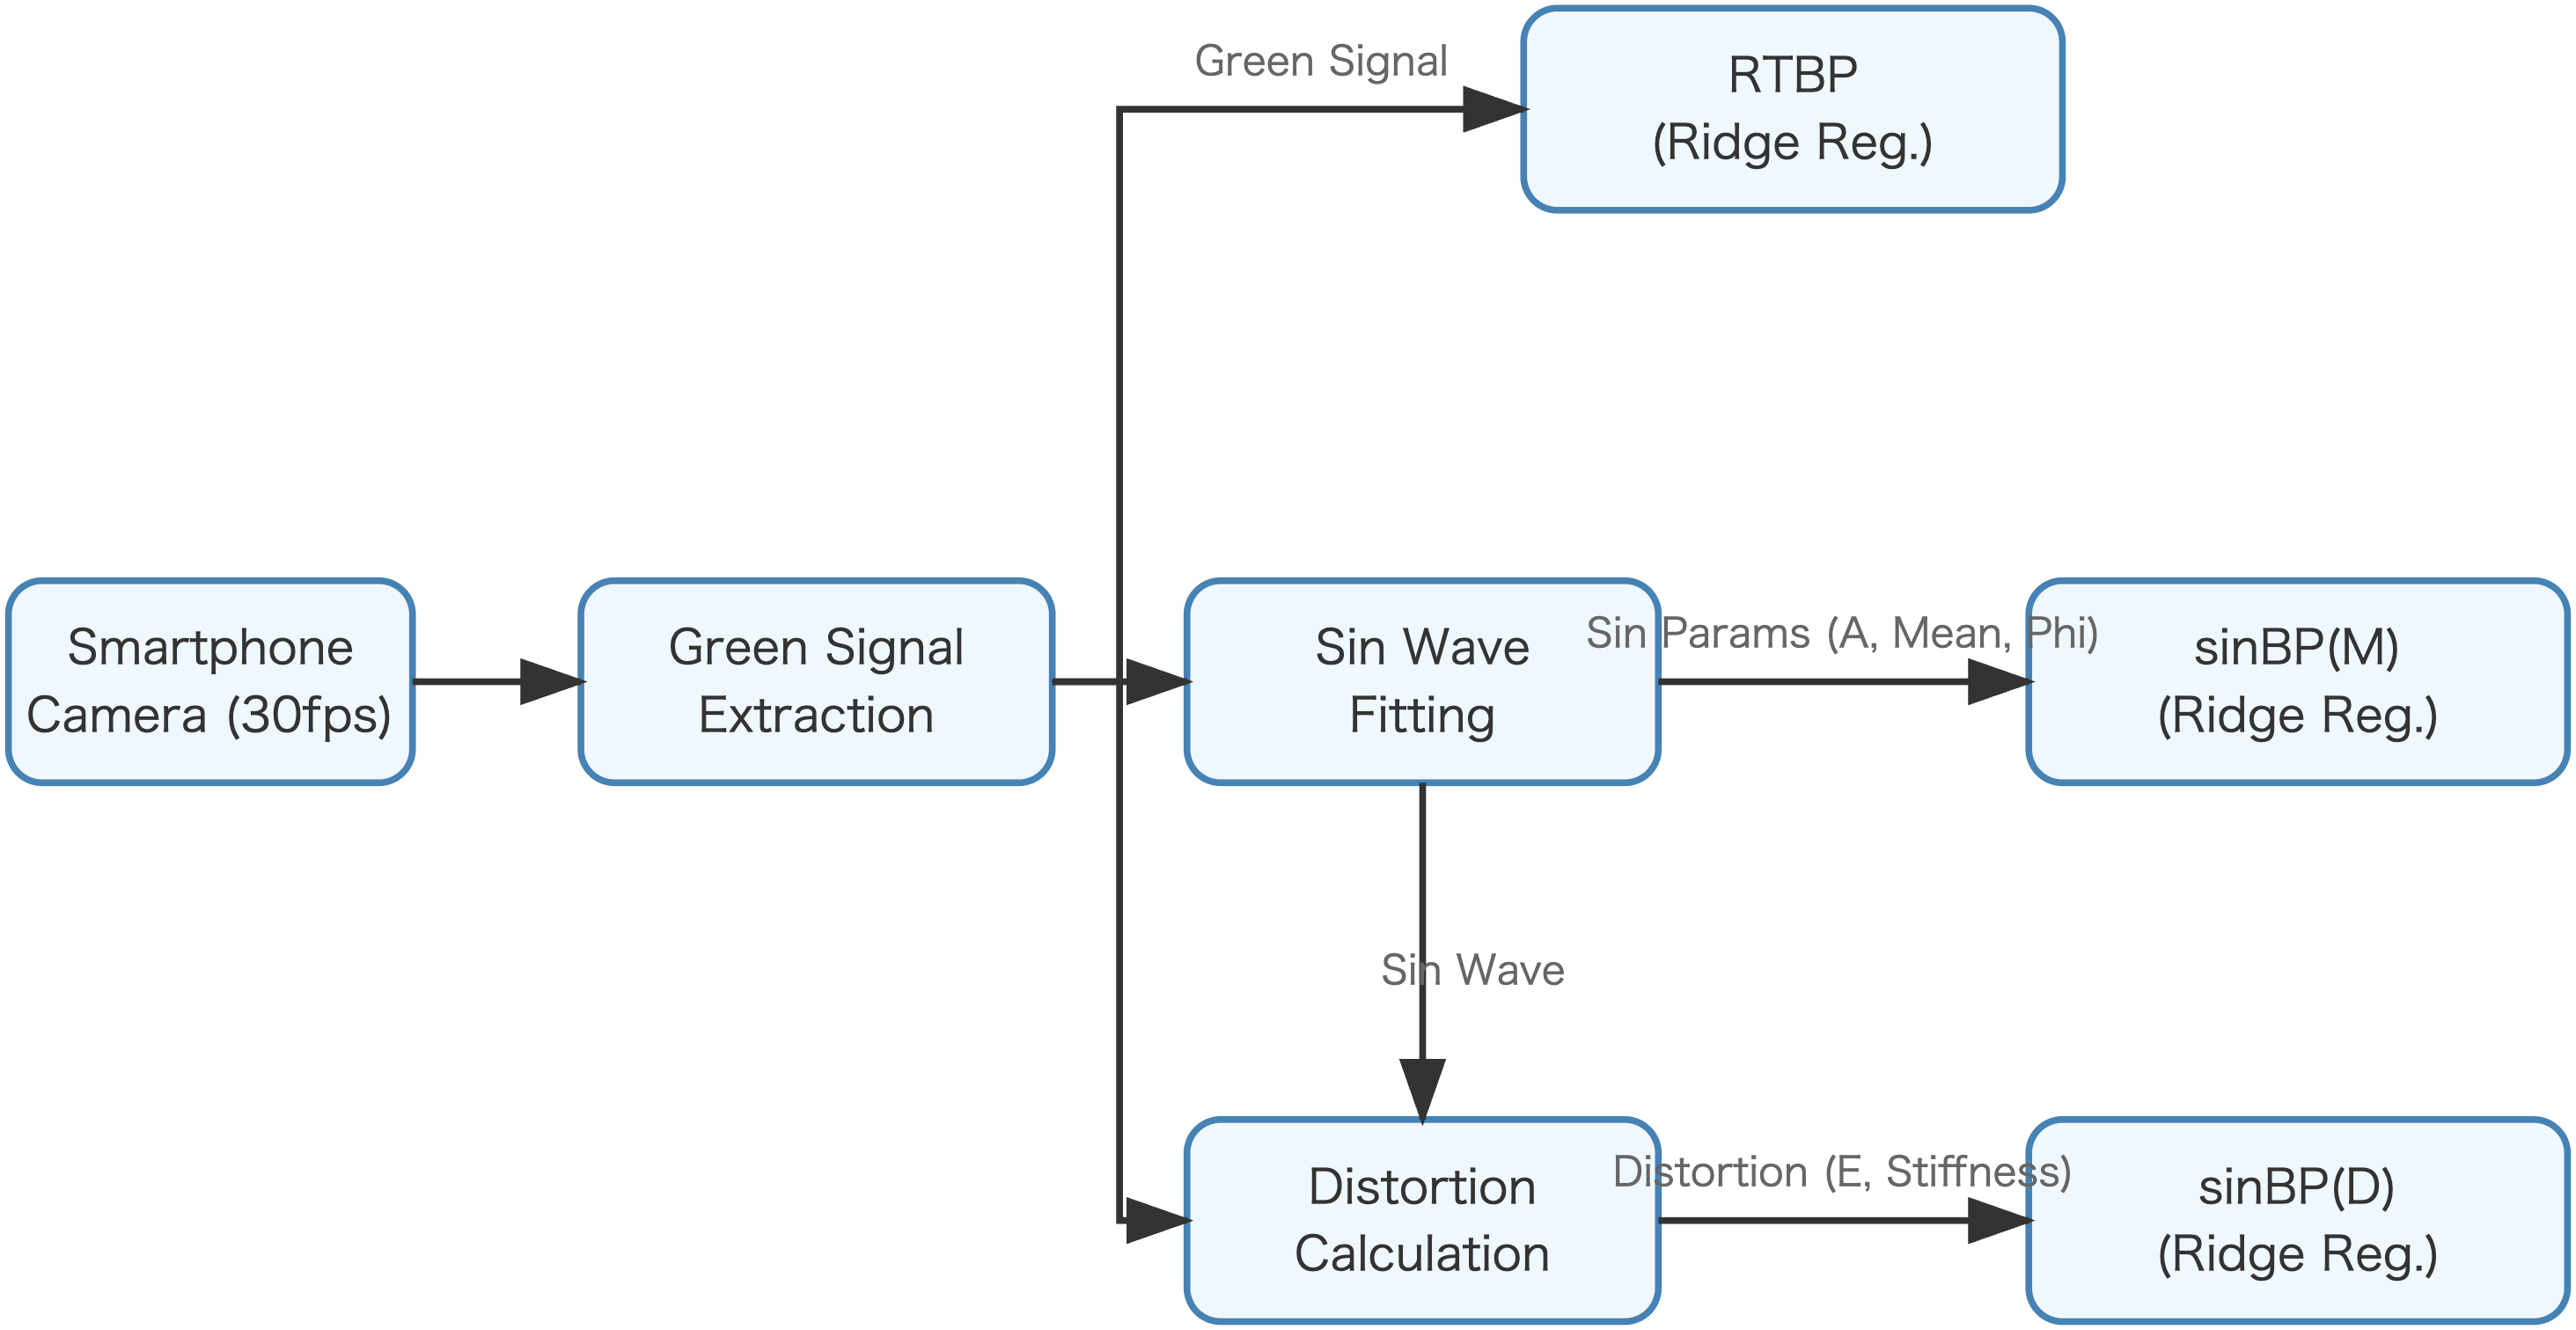
\includegraphics[width=\linewidth]{Fig2}
\caption{Processing overview. The same preprocessed beat sequence is evaluated by the baseline RTBP model and the two asymmetric-sine-based estimators.}
\label{fig:overview}
\end{figure}

\subsection{Asymmetric Sine Wave Model}
The fitted waveform model is defined as
\begin{equation}
s(t) = \mu + \frac{A}{2}\sin(\theta(t)),
\label{eq:model}
\end{equation}
where $A$ is the beat amplitude and $\mu$ is the beat mean. To reflect the short systolic rise and long diastolic decay of a PPG pulse, the phase is described by a piecewise mapping:
\begin{equation}
\theta(t) =
\begin{cases}
-\dfrac{\pi}{2} + \pi\dfrac{t'}{T_{\mathrm{sys}}}, & 0 \le t' < T_{\mathrm{sys}},\\[6pt]
\dfrac{\pi}{2} + \pi\dfrac{t' - T_{\mathrm{sys}}}{T_{\mathrm{dia}}}, & T_{\mathrm{sys}} \le t' < T,
\end{cases}
\label{eq:phase}
\end{equation}
where $T = T_{\mathrm{sys}} + T_{\mathrm{dia}}$ is the beat interval and $t'$ is the intra-beat time after beat alignment. This simple shape was chosen because it preserves the main asymmetry of the pulse waveform while keeping the parameter count low enough for stable fitting in a 30 fps environment.

After fitting, the residual feature is computed as the root-mean-square error between the measured beat $x[n]$ and the fitted model $s[n]$:
\begin{equation}
E = \sqrt{\frac{1}{N}\sum_{n=1}^{N}(x[n]-s[n])^{2}}.
\label{eq:residual}
\end{equation}
In this paper, $E$ is treated as the main interpretable residual feature because it directly measures how much the observed pulse deviates from the smoothed model waveform.

\subsection{Compared Estimators}
Table~\ref{tab:methods} summarizes the three estimators.

\begin{table}[t]
\caption{Compared BP estimators}
\label{tab:methods}
\centering
\footnotesize
\begin{tabular}{>{\raggedright\arraybackslash}p{1.45cm} >{\raggedright\arraybackslash}p{2.2cm} >{\raggedright\arraybackslash}p{3.0cm}}
\toprule
Method & Features & Purpose \\
\midrule
RTBP & Amplitude, heart rate, relative rise time, relative fall time & Morphology-based baseline using point-derived features \\
sinBP(M) & Fitted amplitude, heart rate, mean, phase & Whole-wave model with low-parameter global descriptors \\
sinBP(D) & RTBP amplitude, heart rate, relative rise/fall time, residual $E$ & Residual-aware hybrid estimator using morphology plus asymmetric-sine mismatch \\
\bottomrule
\end{tabular}
\end{table}

All three models use linear regression after the shared preprocessing pipeline and the same reference BP measurements. In the present manuscript, sinBP(D) follows the current Android/PPTX logic, namely the RTBP feature set augmented by the residual $E$. This definition is intentionally simpler than the earlier experimental variant that also included a stiffness-like term.

\subsection{Trend-Oriented Target Definition}
For absolute-BP evaluation, the target is the reference cuffless BP value $y_i$ at beat $i$. For the trend-oriented reanalysis, the target is centered within each recording group:
\begin{equation}
\tilde{y}_i = y_i - \bar{y}_{g(i)},
\end{equation}
where $g(i)$ denotes the recording group of beat $i$ and $\bar{y}_{g(i)}$ is that group's mean SBP or DBP. This target removes between-group level offsets and asks whether each method can track within-recording deviation around the local mean.

For grouped trend evaluation, beats were further averaged within each recording group using non-overlapping time windows. If beat $i$ occurred at elapsed time $t_i$, its window index was defined as
\begin{equation}
w_i = \left\lfloor \frac{t_i}{\Delta} \right\rfloor ,
\end{equation}
where $\Delta$ is the window length in seconds. All predictions and references in the same $(g,w)$ pair were averaged before metric calculation. The representative grouped trend results reported below use GroupKFold and $\Delta=20$~s because this setting balanced error reduction and positive SBP correlation in the current scans.

\subsection{Data Acquisition and Evaluation}
Measurements were acquired with a Google Pixel 8 front camera at 30 fps under controlled indoor illumination of approximately 400 lux. Reference BP was recorded with a CNAP continuous monitor, and a fingertip optical PPG device was used as the waveform reference. The prepared training dataset available in the repository contains 1113 extracted beats in total, of which 469 beats have synchronized reference SBP and DBP values and are used for the BP evaluation reported here. The dataset metadata identify 25 recording-group IDs. This draft reports the prepared-dataset evaluation directly and therefore avoids making stronger claims about the participant structure than can be verified from the current exported files.

Outlier processing in the current training script removes invalid BP references, values outside fixed SBP/DBP ranges, and subject-wise statistical outliers based on a $\pm 3\sigma$ rule. The observed BP range in the prepared dataset was 72.01--191.47 mmHg for SBP and 40.00--123.01 mmHg for DBP. Waveform quality was evaluated by comparing the raw Green-channel waveform and the fitted waveform against the reference PPG using MAPE, MAE, RMSE, and correlation. Absolute BP estimation accuracy was evaluated with five-fold time-series cross-validation so that the current results remain comparable to the stored repository workflow. To judge whether the same representation remained useful under a stricter interpretation, we additionally re-analyzed the cleaned dataset with recording-group-aware GroupKFold validation and with the group-centered trend target defined above. These additional analyses are used in the Discussion to determine which claim is scientifically defensible.

\section{Results}
\subsection{Waveform-Level Effect of Model Fitting}
Table~\ref{tab:waveform} shows that the asymmetric sine fit improved all waveform metrics relative to the raw Green-channel signal. The largest gain was observed in MAPE, which decreased from 29.71\% to 18.22\%. The correlation remained low, indicating that the fitted waveform should be viewed as a smoothing representation rather than a high-fidelity reconstruction of every local pulse detail.

\begin{table}[t]
\caption{Waveform evaluation}
\label{tab:waveform}
\centering
\footnotesize
\begin{tabular}{lcccc}
\toprule
Channel & MAPE [\%] & MAE & RMSE & Corr \\
\midrule
sinWave & 18.22 & 1.82 & 2.24 & 0.19 \\
Green & 29.71 & 2.97 & 3.64 & 0.07 \\
\bottomrule
\end{tabular}
\end{table}

\begin{figure}[t]
\centering
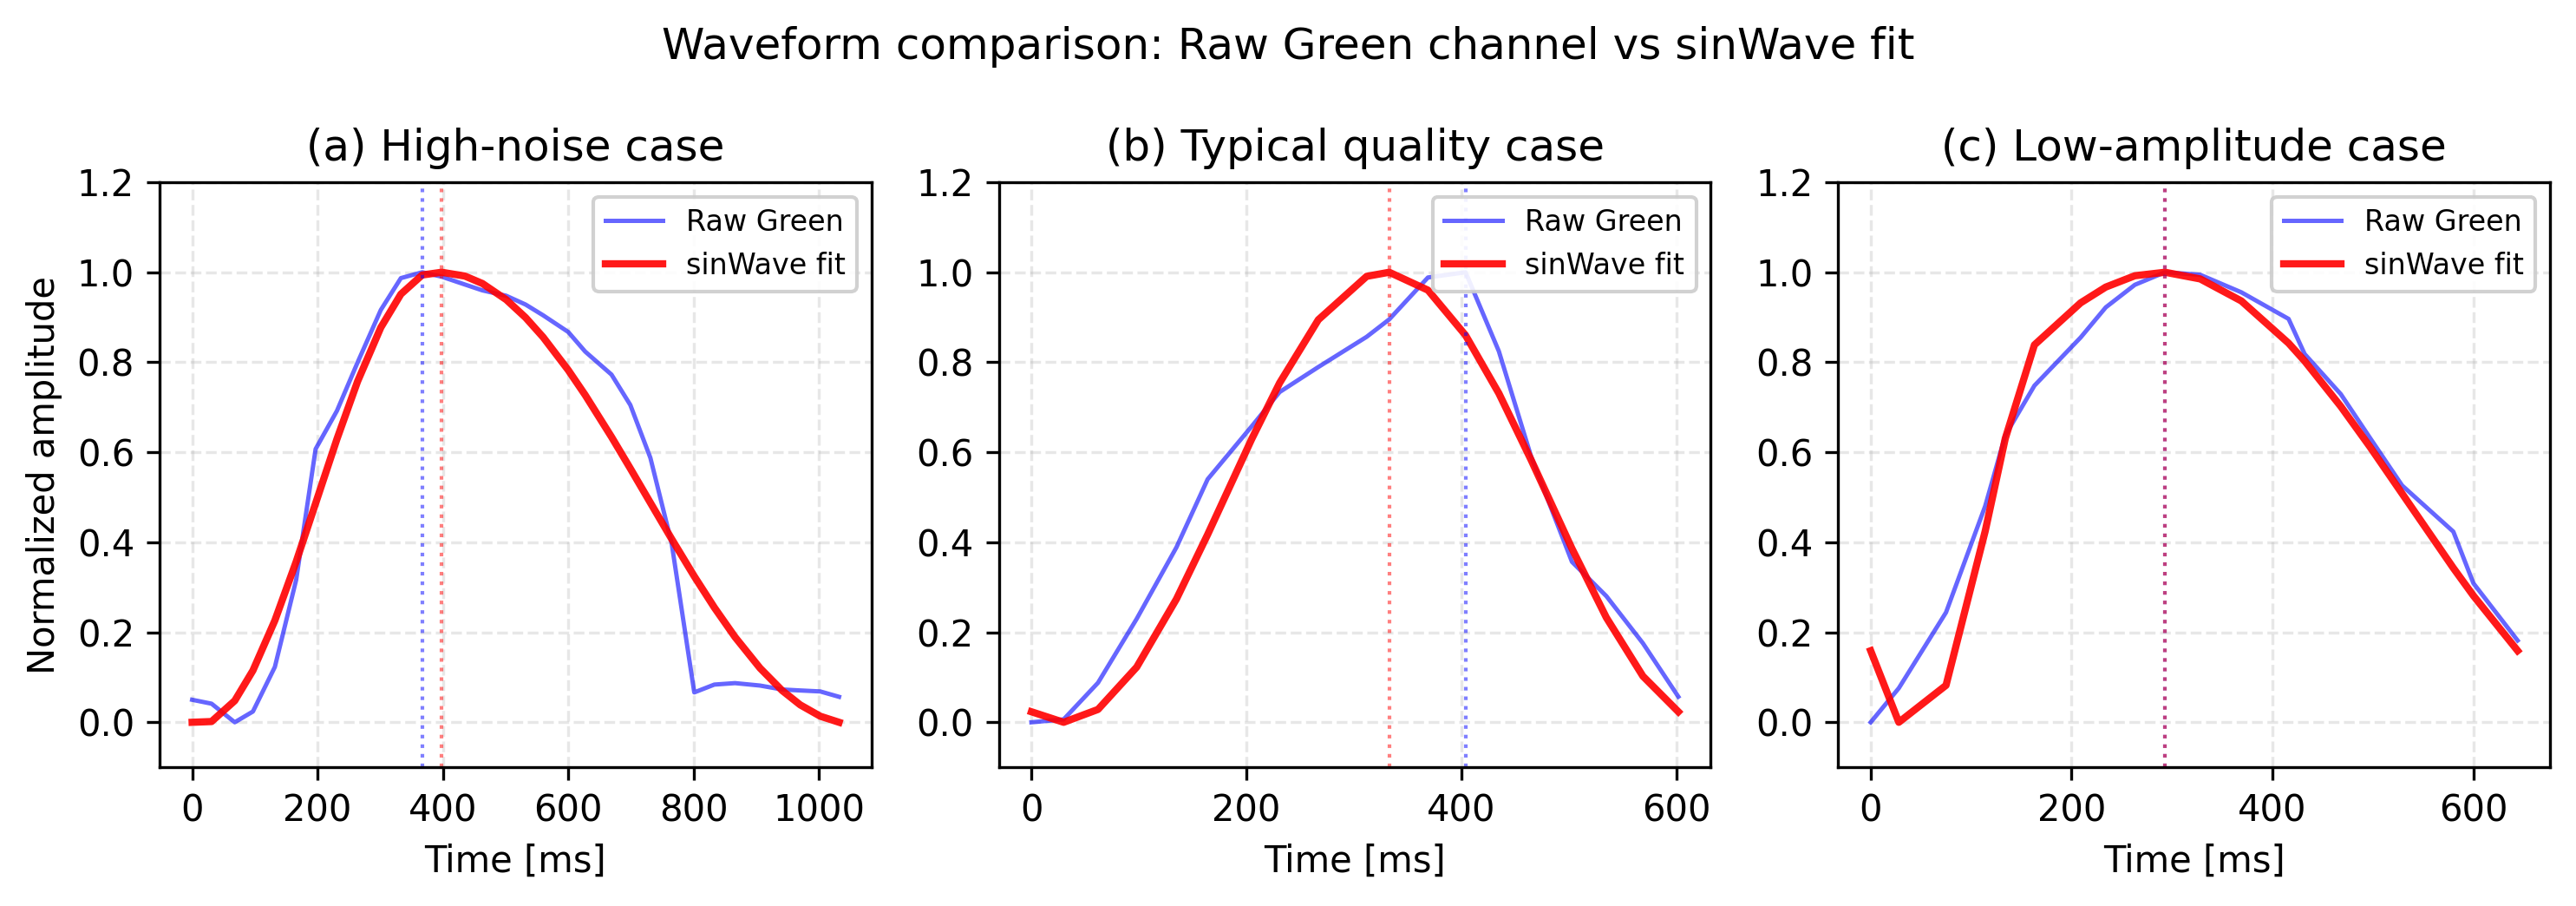
\includegraphics[width=\linewidth]{Fig1}
\caption{Representative beats before and after asymmetric-sine fitting. The fitted waveform suppresses local fluctuation while preserving the coarse beat asymmetry.}
\label{fig:waveform}
\end{figure}

\subsection{Blood Pressure Estimation Accuracy}
Table~\ref{tab:bp_results} summarizes the cleaned five-fold time-series results for absolute BP estimation. Among the three estimators, sinBP(D) achieved the lowest mean MAE and RMSE for both SBP and DBP. Relative to RTBP, the MAE reduction was 1.73 mmHg for SBP and 1.33 mmHg for DBP. However, the fold-to-fold standard deviations were non-negligible, and the correlation coefficients remained modest. These numbers support only a limited statement: within the repository-style time-series evaluation, the residual-aware representation was more stable than the point-feature baseline.

\begin{table*}[t]
\caption{Blood pressure estimation results obtained from the stored five-fold time-series cross-validation outputs}
\label{tab:bp_results}
\centering
\footnotesize
\begin{tabular}{lcccccccc}
\toprule
& \multicolumn{4}{c}{SBP} & \multicolumn{4}{c}{DBP} \\
\cmidrule(lr){2-5}\cmidrule(lr){6-9}
Method & MAPE [\%] & MAE [mmHg] & RMSE [mmHg] & Corr & MAPE [\%] & MAE [mmHg] & RMSE [mmHg] & Corr \\
\midrule
RTBP & 17.84 & 20.68 & 28.08 & -0.06 & 23.17 & 16.13 & 22.51 & 0.17 \\
sinBP(M) & 16.94 & 19.49 & 24.73 & 0.17 & 22.32 & 15.21 & 19.76 & 0.26 \\
sinBP(D) & 16.43 & 18.96 & 24.16 & 0.22 & 21.67 & 14.80 & 19.28 & 0.28 \\
\bottomrule
\end{tabular}
\end{table*}

The improvement was not uniform across all recording groups. Existing subject-level analysis files in the repository show heterogeneous outcomes, and some groups favor RTBP or sinBP(M) instead of sinBP(D). Re-analysis with recording-group-aware validation also showed that absolute cross-group estimation remained weak, especially for SBP. In other words, the time-series results are useful for comparing representations within the prepared dataset, but they are not strong evidence that absolute BP can already be generalized across unseen recording groups.

\subsection{Trend-Oriented Reanalysis}
To identify a claim that is better matched to the current data, we re-analyzed the cleaned dataset from a trend-oriented viewpoint. Instead of asking whether the model could recover the absolute BP level of an unseen group, we asked whether it could more stably follow within-recording BP variation after removing each recording group's mean level. This reanalysis preserved the same three-method comparison, but it used recording-group-aware validation and non-overlapping time-window averaging within each recording group.

Table~\ref{tab:trend_results} summarizes the representative GroupKFold results with 20~s windows. This reframing changed the interpretation of the results. For absolute BP, grouped validation yielded weak SBP performance across methods, indicating that between-group level differences dominated the task. For within-recording SBP trend estimation, however, whole-wave fitting became more convincing. sinBP(D) achieved the lowest SBP trend MAE and RMSE, reaching 3.22/3.90~mmHg with a positive mean correlation of 0.19. For DBP, the centered errors also decreased after time-window averaging, but the ranking between RTBP, sinBP(M), and sinBP(D) remained closer. These findings suggest that the current dataset supports a trend-tracking interpretation more strongly than an absolute-estimation interpretation.

Figure~\ref{fig:trend_scan} places the 20~s result in the broader window-length scan. Longer within-group averaging reduced MAE for all methods, which is expected because short-term beat noise is suppressed. However, the longest window was not automatically the most interpretable setting. For centered SBP, 30~s windows gave the lowest MAE for all methods, but sinBP(D) lost its positive correlation. The 20~s setting was therefore retained as the main grouped-trend condition because it reduced error while preserving a positive SBP correlation and a consistent gap over RTBP.

\begin{table*}[t]
\caption{Group-centered trend results under recording-group-aware GroupKFold with 20~s non-overlapping windows}
\label{tab:trend_results}
\centering
\footnotesize
\begin{tabular}{lcccccccc}
\toprule
& \multicolumn{4}{c}{Centered SBP} & \multicolumn{4}{c}{Centered DBP} \\
\cmidrule(lr){2-5}\cmidrule(lr){6-9}
Method & MAE [mmHg] & RMSE [mmHg] & Corr & MAE SD & MAE [mmHg] & RMSE [mmHg] & Corr & MAE SD \\
\midrule
RTBP & 3.35 & 4.03 & 0.12 & 2.21 & 2.84 & 3.51 & 0.18 & 1.13 \\
sinBP(M) & 3.51 & 4.45 & -0.35 & 1.97 & 2.75 & 3.43 & -0.16 & 1.13 \\
sinBP(D) & 3.22 & 3.90 & 0.19 & 2.23 & 2.88 & 3.58 & 0.06 & 1.32 \\
\bottomrule
\end{tabular}
\end{table*}

\begin{figure}[t]
\centering
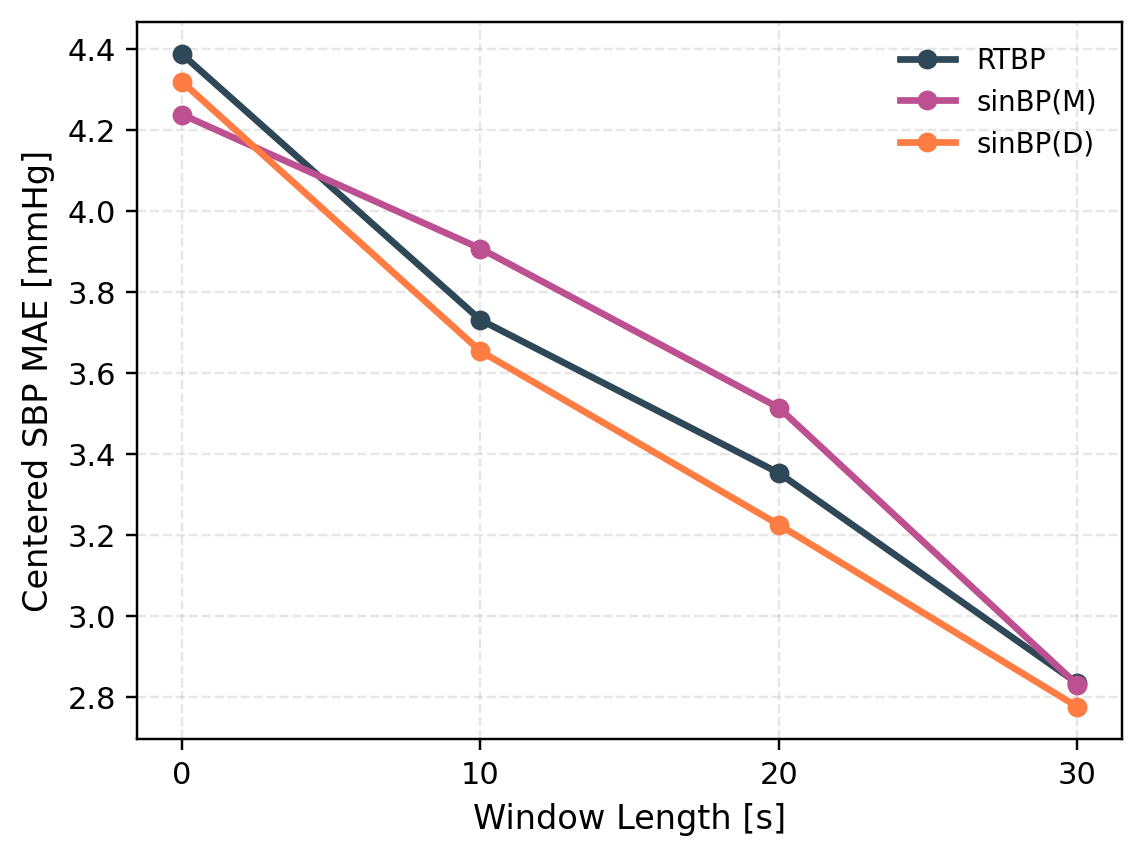
\includegraphics[width=\linewidth]{Fig5}
\caption{Window-length scan for centered SBP under recording-group-aware GroupKFold. sinBP(D) remains below RTBP at 10, 20, and 30~s. The 20~s setting is the shortest window that combines lower error with a positive mean SBP correlation.}
\label{fig:trend_scan}
\end{figure}

\section{Discussion}
\subsection{Why Whole-Wave Fitting Helps at 30 fps}
The main practical advantage of the asymmetric sine approach is that it replaces unstable point picking with beat-wise curve fitting. When the sampling interval is 33 ms, even a small phase shift changes the apparent peak location substantially. A whole-wave fit distributes this uncertainty across the beat and therefore yields more stable descriptors than peak-only morphology.

\subsection{Why the Residual Helps}
The residual term $E$ measures how strongly the observed beat deviates from the smooth asymmetric sine template. In the current implementation, it is appended to the RTBP feature set rather than replacing that set. This additive form should be interpreted as the simplest residual-aware extension of RTBP, not as a proven optimal way to combine residual information with morphology. The available results indicate that this hybrid feature set is associated with lower aggregate error than the point-feature baseline in the repository-style comparison, but the present data do not isolate the specific causal contribution of $E$ alone. Any physiological interpretation should therefore remain tentative.

\subsection{Limitations and Journal-Extension Targets}
The present results remain far from clinical deployment standards. The absolute-estimation results are especially limited by strong between-group level differences, and the correlation values show that beat-to-beat tracking is still weak when the task is defined as direct absolute SBP prediction. In addition, the current draft relies partly on stored repository outputs produced with time-series cross-validation rather than a fully subject-independent split. This is adequate for documenting the present implementation, but insufficient for a strong absolute-generalization claim.

Three expansion items are especially important for journal-level validation. First, a grouped or leave-one-subject-out evaluation should replace the current time-series split as the primary validation for any absolute-BP claim. Second, the participant and recording metadata should be documented explicitly so that the effective sample structure is clear. Third, if the paper adopts the trend-oriented interpretation suggested by the current data, that interpretation should be formalized with clearer protocol labels, failure-case plots, and a direct comparison between absolute and centered targets.

\section{Conclusion}
In the stored repository evaluation for 30 fps visible-light rPPG, whole-wave fitting produced cleaner beat representations than the raw Green-channel waveform and improved aggregate BP-estimation error relative to the point-feature baseline. Among the three compared estimators, the residual-aware fitted-wave model sinBP(D) achieved the lowest mean MAE and RMSE in the current time-series cross-validation outputs.

Taken together with the additional grouped reanalysis, these results support a narrower but more defensible conclusion: compact whole-wave descriptors are promising for low-frame-rate rPPG-based BP trend estimation within recordings, but they do not yet support strong claims about absolute cross-group BP estimation. Stronger validation requires explicit participant metadata, grouped evaluation as the primary protocol, and broader experiments beyond the current prepared dataset.

\bibliographystyle{unsrt}
\bibliography{references}

\end{document}
